%%%%%%%%%%%%%%%%%%%%%%%%%%%%%%%%%%%%%%%%%
% Structured General Purpose Assignment
% LaTeX Template
%
% This template has been downloaded from:
% http://www.latextemplates.com
%
% Original author:
% Ted Pavlic (http://www.tedpavlic.com)
%
% Note:
% The \lipsum[#] commands throughout this template generate dummy text
% to fill the template out. These commands should all be removed when 
% writing assignment content.
%
%%%%%%%%%%%%%%%%%%%%%%%%%%%%%%%%%%%%%%%%%

%----------------------------------------------------------------------------------------
%   PACKAGES AND OTHER DOCUMENT CONFIGURATIONS
%----------------------------------------------------------------------------------------

\documentclass{article}

\usepackage{fancyhdr} % Required for custom headers
\usepackage{lastpage} % Required to determine the last page for the footer
\usepackage{extramarks} % Required for headers and footers
\usepackage{graphicx} % Required to insert images
\usepackage{lipsum} % Used for inserting dummy 'Lorem ipsum' text into the template

\usepackage[T1]{fontenc} % Codificación de las fuentes utilizadas
\usepackage[spanish]{babel} % Español como idioma principal del texto (permite hyphenation de palabras al final de una línea)
\selectlanguage{spanish}
\usepackage{hyperref}
\usepackage{listings}

\usepackage[T1]{fontenc} % Codificación de las fuentes utilizadas
\usepackage[spanish]{babel} % Español como idioma principal del texto (permite hyphenation de palabras al final de una línea)


\usepackage{graphicx}
\usepackage{url}

\graphicspath{{Figures/}{Diagrams}{Chapters/}}  % Location of the graphics files (set up for graphics to be in PDF format)

\selectlanguage{spanish}

\setcounter{tocdepth}{1}

% Include any extra LaTeX packages required
\usepackage[square, numbers, comma, sort&compress]{natbib}  % Use the "Natbib" style for the references in the Bibliography
\usepackage{verbatim}  % Needed for the "comment" environment to make LaTeX comments
\usepackage{vector}  % Allows "\bvec{}" and "\buvec{}" for "blackboard" style bold vectors in maths
\hypersetup{urlcolor=blue, colorlinks=true}  % Colours hyperlinks in blue, but this can be distracting if there are many links.
\usepackage{hyperref}
% \usepackage[pdfauthor={Diego Martín Arroyo},
%             pdftitle={Diseño e implementación de un sistema de computación distribuida con
% Raspberry Pi, y estudio comparativo del mismo frente a otras soluciones},
%             pdfsubject={Memora del Trabajo de Fin de Grado},
%             pdfproducer={XeLaTeX with hyperref},
%             pdfcreator={XeLaTeX},
%             pdfkeywords={Computación Paralela, Sistema Distribuido, Raspberry}
%             ]{hyperref}
%% ----------------------------------------------------------------

%% --------------------------------------------------------------------------------------------------------------------------------
%http://tex.stackexchange.com/a/85218/76599
\usepackage{fancyvrb}
\usepackage[dvipsnames]{xcolor}

% redefine \VerbatimInput
\RecustomVerbatimCommand{\VerbatimInput}{VerbatimInput}% Inclusión de archivos de texto plano
{fontsize=\footnotesize,
 %
 frame=lines,  % top and bottom rule only
 framesep=2em, % separation between frame and text
 rulecolor=\color{Gray},
 %
 label=\fbox{\color{Black}data.txt},
 labelposition=topline,
 %
 commandchars=\|\(\), % escape character and argument delimiters for
                      % commands within the verbatim
 commentchar=*        % comment character
}

\usepackage{listings} % Requerido para la inserción de código
%Listings command

\usepackage{float}
\newcommand*\lstinputpath[1]{\lstset{inputpath=#1}}
\lstinputpath{Code/}

\newcounter{undefinedreferences}
\setcounter{undefinedreferences}{0}

\newcommand{\citationneeded}[1][None]{\stepcounter{undefinedreferences}\textsuperscript{\color{blue} [Citation needed: #1]}}

\newcommand{\checkreferences}{
\ifnum\value{undefinedreferences} > 0
\begin{center}
\immediate\write18{wget -O Figures/protester.png -nc http://imgs.xkcd.com/comics/wikipedian_protester.png}
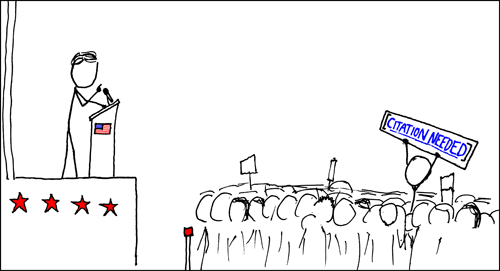
\includegraphics[width=\textwidth]{protester.png}\\
There are \arabic{undefinedreferences} undefined references
\end{center}
\else
No undefined references. Good!
\fi
}


%https://github.com/pads-fhs/LaTeX-Template-Thesis/blob/master/lststyles.tex
\lstdefinelanguage{JavaScript}{
  keywords={typeof, new, true, false, catch,%
    function, return, null, catch, switch, var,%
    if, in, while, do, else, case, break},
  ndkeywords={class, export, boolean, throw, implements, import, this},
  sensitive=false,
  comment=[l]{//},
  morecomment=[s]{/*}{*/},
  morestring=[b]',
  morestring=[b]"
}
\newcommand{\lstsetjavascript}{
  \lstset{
		language=JavaScript,
		breaklines=true,
		commentstyle=\textit,
		basicstyle=\ttfamily,
		keywordstyle=\bfseries,
		stringstyle=\ttfamily,
		showstringspaces=false,
		frame=single,
		tabsize=2
  }
}

\lstdefinelanguage{log}{
  keywords={typeof, new, true, false, catch,%
    function, return, null, catch, switch, var,%
    if, in, while, do, else, case, break},
  ndkeywords={class, export, boolean, throw, implements, import, this},
  sensitive=false,
  comment=[l]{//},
  morecomment=[s]{/*}{*/},
  morestring=[b]',
  morestring=[b]"
}
\newcommand{\lstsetlog}{
  \lstset{
		language=log,
		breaklines=true,
		commentstyle=\textit,
		basicstyle=\ttfamily,
		keywordstyle=\bfseries,
		stringstyle=\ttfamily,
		showstringspaces=false,
		frame=single,
		tabsize=2
  }
}

\lstloadlanguages{Java,XML, JavaScript, log}

\newcommand{\javascriptcode}[4]{
	\lstinputlisting[caption=#2,label=#1, firstline=#3, lastline=#4]{#1.json}
}

\newcommand{\logcode}[4]{
	\lstinputlisting[caption=#2,label=#1, firstline=#3, lastline=#4]{#1.log}
}

\usepackage[bottom]{footmisc} %The footnotes go at the bottom of t\usepackage{dtklogos}he page, instead next to the last line.
%Ajustes para Java
% \lstset{
% 	language=java,
%  	frame=single, % Un marco simple alrededor del código
%     basicstyle=\small\ttfamily, % Utilizar fuente true type pequeña
%     keywordstyle=[1]\color{Blue}\bf, % Funciones en negrita y azul
%     keywordstyle=[2]\color{Purple}, % Argumentos en morado
%     keywordstyle=[3]\color{Blue}\underbar, % Funciones personalizadas subrayadas en azul
%     identifierstyle=, % Nada especial acerca de identificadores
%     commentstyle=\usefont{T1}{pcr}{m}{sl}\color{Green}\small, % Los comentarios se renderizan en fuente pequeña verde
%     stringstyle=\color{Purple}, % Cadenas en morado
%     showstringspaces=false, % No se muestran los espacios entre cadenas
%     tabsize=5, % 5 espacios por tabulado
%     %
%     % Put standard Perl functions not included in the default language here
%     %morekeywords={rand},
%     %
%     % Put Perl function parameters here
%     %morekeywords=[2]{on, off, interp},
%     %
%     % Put user defined functions here
%     %morekeywords=[3]{test},\usepackage{dtklogos}
%    	%
%     morecomment=[l][\color{Blue}]{...}, % Line continuation (...) like blue comment
%     numbers=left, % Número de línea a la izquierda
%     firstnumber=1, % Número de línea comienza en 1
%     numberstyle=\tiny\color{Blue}, % Los números de línea son azules y pequeños
%     stepnumber=5, % Los números de línea van de 5 en 5
%     breaklines=true % Salto de línea si el texto no entra. See http://stackoverflow.com/a/1875803
% }

%\usepackage{xltxtra} % XeLaTeX logo. Yep, just that
%http://tex.stackexchange.com/a/73179/76599
\usepackage{metalogo}
%\usepackage{dtklogos} %BibTeX logo
\def\BibTeX{{\rm B\kern-.05em{\sc i\kern-.025em b}\kern-.08em
    T\kern-.1667em\lower.7ex\hbox{E}\kern-.125emX}}

\newenvironment{alignedDescription}[2][0pt]
  {\begin{list}{}%
    {\renewcommand\makelabel[1]{\textsf{\textbf{##1}}\hfil}%
     \settowidth\labelwidth{\makelabel{#2}}%
     \setlength\leftmargin{\labelwidth+\labelsep + #1}}}%
  {\end{list}}

\newenvironment{elements}
{\begin{quote}\itshape\centering\small}
{\end{quote}}

\newenvironment{cabstract}
{\begin{quote}\itshape\centering\small}
{\end{quote}}

%\usepackage[xindy]{glossaries}
%\newcommand{\chapterabstract}{1}{
%	\begin{center}
%	\small\textit
%	#1
%	\end{center}
%}

\usepackage{xcolor,colortbl}
\usepackage{float}
%----------------------------------------------------------------------------------------
%   NAME AND CLASS SECTION
%----------------------------------------------------------------------------------------

\newcommand{\hmwkTitle}{Requisitos software} % Assignment title
\newcommand{\hmwkDueDate}{Miércoles,\ 13\ de\ mayo\ de\ 2015} % Due date
\newcommand{\hmwkAuthorName}{Diego Martín Arroyo} % Your name

\graphicspath{{Figures/}}
%----------------------------------------------------------------------------------------
%   TITLE PAGE
%----------------------------------------------------------------------------------------

\title{\hmwkTitle}
\author{\textbf{\hmwkAuthorName}}
\date{\hmwkDueDate}

%----------------------------------------------------------------------------------------



\begin{document}

\maketitle
\begin{abstract}

La definición de los requisitos de una herramienta \textit{software} facilita la comprensión por parte de todas las partes implicadas de los aspectos relevantes del mismo, además de facilitar la planificación del desarrollo del mismo con un grado de certeza mayor. El presente documento recoge los objetivos del sistema desde un enfoque basado en las necesidades de los diferentes usuarios del mismo, atendiendo a los diferentes roles desarrollados y los resultados de las diversas evaluaciones realizadas. 
\end{abstract}
%----------------------------------------------------------------------------------------
%   TABLE OF CONTENTS
%----------------------------------------------------------------------------------------

\setcounter{tocdepth}{1}

\tableofcontents
\newpage

\section{Introducción}

% El uso de un sistema conformado por varios nodos dificulta su mantenimiento, y en particular la instalación de un conjunto de herramientas iniciales y las posteriores actualizaciones. Dicho mantenimiento, si es llevado a cabo de forma ``manual'' suele propiciar fallos humanos. Por ello, en el desarrollo del sistema se ha apostado por una herramienta que automatice la instalación del sistema operativo reduciendo al máximo el tiempo de atención que el administrador debe prestar a cada nodo.

% En el presente documento se detallan las decisiones de usuario llevadas a cabo en el desarrollo de la utilidad \textbf{marco-netinst}, que lleva a cabo este cometido, así como el funcionamiento de dicha herramienta.

\section{Formato}

El formato utilizado durante el desarollo de la presente especificación se ajusta al dispuesto por el estándar \textbf{830-1998} del IEEE.

%TODO: Mantiene por tanto los principios de no ambigüedad


%TODO: La especificación de requisitos ha sido evaluada por una tercera parte, a fin de evaluar la concreción de los diferentes apartados

\section{Objectivos del proyecto}

%TODO: Complete with the main.tex data

\section{Usuarios participantes}

El sistema debe integrarse en una infraestructura ya existente con una serie de usuarios fácilmente identificables cuyos roles ya se encuentran claramente definidos.

\subsection{Usuarios principales}

Son Usuarios Principales aquellos cuya interacción con el sistema se basa en la explotación de los servicios que ofrece el mismo. No son responsables, por tanto, de las diferentes tareas de gestión, administración y mantenimiento del sistema.

\subsubsection{Estudiantes}

Uno de los objetivos del sistema es la integración del mismo en un contexto universitario, con el objetivo de ser utilizado como herramienta didáctica para el estudio de los paradigmas de computación distribuida y paralela.

\section{Evaluación de alternativas}

Como se define en la memoria del Trabajo, las opciones típicamente utilizadas por administradores de sistemas no son viables en el sistema a construir debido a las características de la plataforma utilizada: los equipos \textbf{Rasbperry Pi} no soportan el protocolo \textbf{PXE}, por lo que es necesario crear una herramienta propia, o buscar alternativas ya existentes creadas para un problema similar.

\subsection{Estrategia inicial}

El arranque de una placa \textbf{Rasbperry Pi} es llevado a cabo principalmente por la GPU de la placa. Al conectarse a la corriente eléctrica, se activa la secuencia de arranque definida en la memoria ROM de la placa. Este código busca en la primera partición de la tarjeta SD un \textit{bootloader} y lo carga, activando la memoria SDRAM y pasando al siguiente estado, en el que se carga el archivo start.elf, encargado de cargar el Kernel del sistema operativo, según los parámetros definidos en los ficheros \texttt{config.txt}, \texttt{cmdline.txt} y \textbf{bcm2835.dtb}.

\begin{figure}[H]
	\centering
	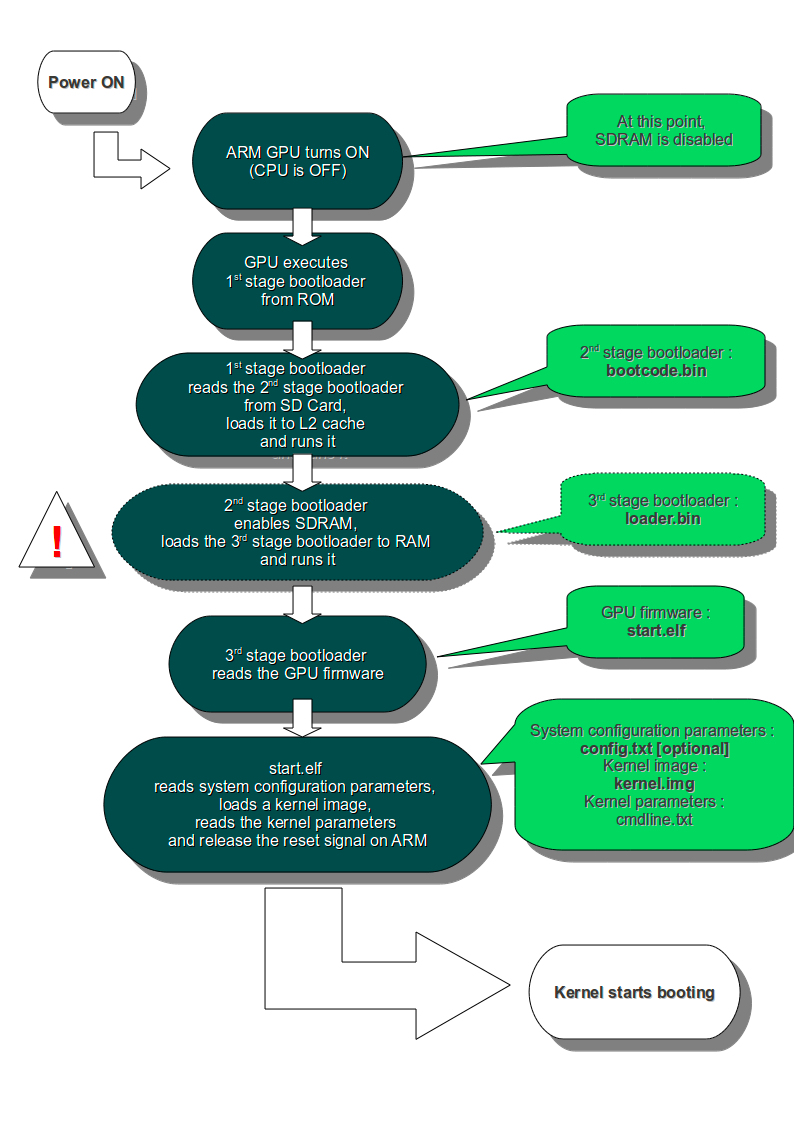
\includegraphics[width=0.4\textwidth]{bootsequence}
	\caption{Secuencia de arranque de la Raspberry Pi\cite{bootsequence}}
	\label{bootsequence}
\end{figure}

Un archivo de configuración \texttt{cmdline.txt} sin modificar suele seguir la siguiente estructura:

\begin{lstlisting}[frame=single,basicstyle=\small\ttfamily]
root=/dev/mmcblk0p2 rw rootwait console=ttyAMA0,115200 console=tty1 \
selinux=0 plymouth.enable=0 smsc95xx.turbo_mode=N dwc_otg.lpm_enable=0 \
kgdboc=ttyAMA0,115200 elevator=noop
\end{lstlisting}

Los parámetros de interés son los siguientes:

\begin{itemize}
	\item \texttt{root}: Partición raíz a utilizar (generalmente la segunda partición)
	\item \texttt{init}: Especifica el archivo a ejecutar en el arranque. Este proceso tendrá por tanto el \textbf{PID} 1 y generalmente su ejecutable es el fichero \texttt{/sbin/init}\footnote{En sistemas donde \texttt{systemd} es el proceso inicial, \texttt{/sbin/init} es un enlace simbólico al ejecutable de \texttt{systemd}}. Si no se especifica, como ocurre en el archivo por defecto, su valor es este\cite{kernelparams:init}.
\end{itemize}

Modificando el parámetro \texttt{init} es posible ejecutar un código diferente a \texttt{init} en el proceso de arranque, que realice la descarga e instalación del sistema operativo, logrando una solución de compromiso entre la instalación manual y el uso de \textbf{PXE}.

Debido a la falta de experiencia en el desarrollo de herramientas similares, se han probado varios enfoques:

\section{Primer enfoque: modificación del script de inicio}

En este primer intento se crea un \textit{script} y un ejecutable programado en C con un conjunto mínimo de utilidades que permitan la descarga del sistema operativo. Estos archivos son instalados en la primera partición de la tarjeta SD, siendo correctamente ejecutados. Sin embargo, no es posible llevar a cabo la instalación debido a la falta de herramientas de configuración de red.

\section{Segundo enfoque: Busybox}

\textbf{Busybox} es una utilidad que aglutina un conjunto de herramientas UNIX en un único ejecutable de tamaño muy reducido, reemplazando así el uso de varios paquetes, como fileutils o shellutils. Las utilidades a las que reemplaza cuentan con mucha menos funcionalidad, pero son capaces de crear un sistema utilizable con únicamente un kernel y varios ficheros de configuración\cite{aboutbusybox}. Es la opción más común a la hora de crear sistemas embebidos o para realizar operaciones sin un sistema operativo.

Utilizando BusyBox es posible configurar la interfaz de red de la Raspberry Pi mediante \textbf{DHCP} gracias a la herramienta \textbf{udhcpc} así como a un conjunto de herramientas de utilidad como \textbf{wget}.\\

Incluyendo BusyBox en el código del primer proyecto es posible conseguir acceso a la red, pero el hecho de no utilizar el proceso \textbf{init} dificulta la mayor parte de operaciones, por lo que esta opción es descartada.

\section{Enfoque definitivo}

Antes de detallar la solución definitiva al problema, es necesario detallar las herramientas de terceros valoradas y descartadas:

\subsection*{Raspi-LTSP, PiNET}

Estos proyectos\cite{raspiltsp, pinet} están enfocados a la centralización de toda la información en un servidor, y delegan la carga del sistema operativo al mismo, por lo que no constituyen una opción viable.

\subsection*{BerryBoot}

BerryBoot\cite{berryboot} es un sistema de arranque que posibilita la descarga e instalación de un sistema operativo y la coexistencia de varios en una misma tarjeta SD. Constituye una opción bastante prometedora, que sin embargo depende significativamente de una interfaz gráfica, haciendo que su uso sea inviable para el objetivo deseado.

\subsection{Propuesta de solución}

El proyecto \textbf{raspbian-ua-netinst}\cite{raspbian-ua-netinst} posibilita la instalación de la distribución Raspbian desde un repositorio público, realizando el particionado de la tarjeta SD, la descarga e instalación de los ficheros y el resto de tareas necesarias desde la propia máquina, únicamente instalando en la tarjeta unos 15 megabytes de información. Este proyecto ha sido adaptado a las necesidades específicas del sistema, con las siguientes modificaciones:

\begin{itemize}
	\item Instalación de \textbf{ArchLinux ARM} en lugar de \textbf{Raspbian}.
	\item Instalación del sistema operativo completo a partir de un archivo \textbf{.tar.gz} en lugar de la descarga de paquetes.
	\item Nuevo \textit{script} de carga del \textit{software} en la tarjeta SD (en el paquete original se delega a utilidades de terceros).
	%TODO\item Posibilidad de aplicar diferentes esquemas de particionado
	\item Detección del servidor sin configuración previa utilizando \textbf{MarcoPolo}.
	%TODO\item Interfaz administrativa de los sistemas operativos ofrecidos
\end{itemize}

El sistema se compone de varios componentes, como se detalla en la siguiente sección.

\section{marco-netinst}

\textbf{marco-netinst} está compuesto por un conjunto de herramientas que permiten la gestión de los nodos del sistema y la instalación del sistema operativo en los mismos. Para ello se compone de varios módulos:

\subsection{marco-netinst}

Este módulo, basado en \textbf{raspbian-ua-netinst} únicamente comprende varios scripts, detallados a continuación:

\subsubsection*{update.sh}

Descarga del repositorio indicado los paquetes que necesita el sistema operativo para arrancar. Dichos paquetes consisten básicamente en código de arranque, \textit{kernels}, bibliotecas y un conjunto de herramientas básicas, siendo la más importante de ellas \textbf{BusyBox}. El \textit{script} realiza la descarga en un directorio temporal de los archivos \textbf{.deb}.

\subsubsection*{build.sh}

Crea los archivos necesarios para la instalación, que deberán ser copiados a la tarjeta SD. Para ello, realiza la siguiente secuencia de acción:

\begin{enumerate}
\item Copia del \textit{kernel}.
\item Creación de los archivos de configuración.
\item Creación de los archivos \textbf{.cpio} (uno por cada arquitectura) que aglutina todas las bibliotecas, ejecutables y otros archivos de interés, así como los \textit{scripts} que llevarán a cabo la instalación del sistema operativo. 
\item Creación de los parámetros de la línea de comandos.
\item Copia de las utilidades de \textbf{MarcoPolo}.
\item Creación de un fichero \textbf{.zip}.
\end{enumerate}

\subsubsection*{deploy.sh}

Formatea la tarjeta SD, creando una única partición, donde descomprime el archivo \textbf{.zip} creado anteriormente.

Estos tres \textit{scripts} deben ser ejecutados en el orden en el que han sido expuestos, pues dependen de los archivos generados por el resto. En caso de que no se realice la llamada de uno sin su antecesor, este procederá a su ejecución antes de realizar la funcionalidad que le corresponde.

\subsubsection*{clean.sh}

Elimina todos los ficheros temporales y el resultado de las ejecuciones.

\subsection{marco-bootstrap}

Ejecutable en C++ que permite llevar a cabo el descubrimiento del servidor donde se aloja el sistema operativo mediante \textbf{MarcoPolo}. Debido a la ausencia del \textit{daemon} de \textbf{Marco} en el sistema, se utiliza una implementación básica del protocolo, denominada \textbf{marco-minimal}. Esta implementación expone la misma funcionalidad que el \textbf{binding} de Marco en C++, pero a más bajo nivel.

\subsection{marco-bootstrap-backend}

Interfaz de gestión de los sistemas operativos que el servidor ofrece para su descarga.

\section{Instalación}

El conjunto de herramientas que realizan la instalación del sistema operativo están basadas en \textbf{Debian}, y por tanto utilizan el gestor de arranque \textbf{init}. Para realizar la instalación por tanto se delegará la ejecución de los \textit{scripts} que realicen las funciones a dicho gestor. Por ello, se define el script \texttt{/etc/rcS}, que es ejecutado en cualquier nivel de ejecución (\textit{runlevel})\footnote{\href{http://apt-browse.org/browse/ubuntu/trusty/main/all/sysv-rc/2.88dsf-41ubuntu6/file/etc/rcS.d/README}{apt-browse.org/browse/ubuntu/trusty/main/all/sysv-rc/2.88dsf-41ubuntu6/file/etc/rcS.d/README}}. 

El script lleva a cabo la siguiente secuencia de tareas:

\begin{enumerate}
	\item Define una serie de variables de utilidad.
	\item Crea de directorios necesarios dentro de la tarjeta SD.
	\item ``Instala'' todas las utilidades de \textbf{BusyBox} (permite el acceso a las mismas) y define las rutas de búsqueda de ficheros mediante la variable \texttt{\$PATH}.
	\item Monta de los pseudosistemas de ficheros \texttt{/proc} y \texttt{/sys}.
	\item Establece mecanismos de redirección de una copia de las salidas estándar y de error (\textbf{stdout} y \textbf{stderr}) a un fichero de log para su posterior análisis.
	\item Determina el tipo de \textit{hardware} sobre el que se está ejecutando el \textit{script}, a fin de instalar versión del sistema operativo apropiada.
	\item Copia los ficheros de arranque contenidos en la tarjeta SD.
	\item Carga un \textit{script} con parámetros adicionales definidos por el usuario.
	\item Configura de la interfaz de red \textbf{eth0} mediante \textbf{DHCP}.
	\item Determina de la hora mediante \textbf{NTP}.
	\item Carga módulos del \textit{kernel} si son necesarios.
	\item Particiona la tarjeta SD según el siguiente esquema:
	\begin{itemize}
		\item Partición 1: 128 megabytes, formato FAT32.
		\item Partición 2: Resto de la tarjeta SD, formato ext4.
	\end{itemize}
	\item Busca de servidores que alojen el sistema operativo mediante \textbf{MarcoPolo}.
	\item Descarga el sistema operativo como archivo \texttt{.tar.gz}.
	\item Descomprime el sistema operativo en la partición número 2 (donde la mayoría de ficheros se almacenan. La estructura del fichero \texttt{.tar.gz} define el lugar donde cada fichero se debe alojar, y los permisos de acceso a los ficheros son conservados en el proceso de extracción, por lo que con la extracción se consigue además la estructuración del sistema y la gestión de permisos).
	\item Mueve los ficheros de arranque a la partición 1 (\textit{kernel}, parámetros de arranque, etcétera).
	\item Ejecuta los \textit{scripts} de post-instalación.
	\item Almacena el fichero de log.
	\item Limpia archivos temporales.
	\item Desmonta los sistemas de ficheros y procede al reinicio del sistema.
\end{enumerate}

Una vez ejecutado el script el nodo está preparado para integrarse en el sistema. El tiempo total de instalación es de unos 5 minutos, según el fichero de log, dependiendo del estado de la red. En pruebas realizadas, el tiempo de descarga supone aproximadamente la mitad del tiempo total de instalación, si bien mejora significativamente cuando se cuenta con un servidor local que aloje el sistema operativo.

\nocite{rpiconfig}

 \label{Bibliography}
 \lhead{\emph{Bibliografía}}  % Change the left side page header to "Bibliography"
 \bibliographystyle{ieeetr}  % Use the "unsrtnat" BibTeX style for formatting the Bibliography
 \bibliography{marcobootstrap}  % The references (distcc) information are stored in the file named "distcc.bib"

\end{document}
